% Group 28 report — LaTeX integration owned by B (Dylan).
% Build: latexmk -pdf main.tex   (from report/)
% Target ~3-4 pages per course spec. Section owners are marked in the stubs.
\documentclass[10pt,a4paper]{article}
\usepackage[margin=2.4cm]{geometry}
\usepackage{amsmath,amssymb}
\usepackage{graphicx}
\usepackage{booktabs}
\usepackage{natbib}
\usepackage[hidelinks]{hyperref}

\newcommand{\R}{\mathbb{R}}
\newcommand{\todo}[1]{\textbf{[TODO: #1]}}

\title{\bfseries Learning with Local and Global Consistency:\\
  Group 28 Report (draft)}
\author{Iliyas Baishev \quad Dylan Porter \quad Surkhay Malikov \quad Karu Thumula\\
  \small COMP3314 Machine Learning, HKU, 2026--27 Sem 1}
\date{Draft --- \today}

\begin{document}
\maketitle
\vspace{-3em}

% Section owned by D (Thumula): motivation, problem setting, consistency assumptions.
\section{Introduction}\label{sec:intro}

\emph{[D to write: the semi-supervised setting, local vs global consistency
assumptions, why the two-moons picture motivates the method. Target $\approx$0.4
page. Placeholder keeps the page budget visible in the draft.] \todo{placeholder}}
          % D
% Section owned by A (Iliyas).
\section{Algorithm}\label{sec:algorithm}

Learning with Local and Global Consistency builds a weighted graph over
both labeled and unlabeled points \citep[Section~2]{zhou2003consistency}.
For distinct points, the Gaussian affinity is
$W_{ij}=\exp(-\lVert x_i-x_j\rVert^2/(2\sigma^2))$, where $\sigma$ controls
how quickly similarity decreases with distance. Setting $W_{ii}=0$
prevents direct self-reinforcement. With the diagonal degree matrix
$D_{ii}=\sum_j W_{ij}$, the method normalizes the affinity at both ends
of each edge by forming $S=D^{-1/2}WD^{-1/2}$.

For $n$ points and $c$ classes, $Y\in\R^{n\times c}$ has one-hot rows for
known labels and zero rows for unlabeled points. Starting with $F^{(0)}=Y$,
the method updates the class scores by
\begin{equation}
  F^{(t+1)}=\alpha SF^{(t)}+(1-\alpha)Y,\qquad 0<\alpha<1.
\end{equation}
The first term collects class scores from neighbors. The second adds the
original label signal back at every round. After several updates, a label
can influence points multiple edges away. This lets unlabeled points along
a curve connect distant points on the same structure. At convergence,
each unlabeled point $i$ is assigned the class with the highest score in
row $i$ of $F^*$. Section~\ref{sec:theory} explains why the iteration
converges and relates it to the regularized objective.
      % A
% Section owned by B (Dylan): theory, convergence, regularization, our checks.
\section{Theory: convergence and regularization}\label{sec:theory}

The iteration of Section~2,
$F(t+1) = \alpha S F(t) + (1-\alpha) Y$ with $S = D^{-1/2} W D^{-1/2}$,
converges because of what the symmetric normalization buys: $S$ is similar to the
row-stochastic matrix $D^{-1}W$, so its eigenvalues share those of a stochastic
matrix, and being symmetric they are real, all in $[-1,1]$ with top eigenvalue
exactly $1$. Hence for $\alpha \in (0,1)$ the spectral radius of $\alpha S$ is
$\alpha < 1$, the Neumann series $\sum_{i\ge 0}(\alpha S)^i = (I - \alpha S)^{-1}$
converges, and iterating from any starting point gives
\begin{equation}
  F^{*} = (1-\alpha)\,(I - \alpha S)^{-1}\, Y ,
  \label{eq:fixedpoint}
\end{equation}
the paper's closed form (its Eq.~3 up to the constant $1-\alpha$, which does not
affect the argmax rule). Writing $F(t) - F^{*} = (\alpha S)^{t}\,(F(0) - F^{*})$
shows both advertised properties at once: the limit is independent of $F(0)$, and
the error decays geometrically at rate $\alpha$.

Equation~\eqref{eq:fixedpoint} is not a lucky coincidence of the iteration; it is
the unique global minimiser of a regularised objective. With
$\mathcal{Q}(F) = \tfrac12 \sum_{i,j} W_{ij}
\bigl\|\tfrac{F_i}{\sqrt{D_{ii}}} - \tfrac{F_j}{\sqrt{D_{jj}}}\bigr\|^{2}
+ \mu \sum_i \|F_i - Y_i\|^{2}$ (the paper's Eq.~4), setting $\partial\mathcal{Q}/\partial F = 0$
gives $F - SF + \mu(F - Y) = 0$, and the substitution $\alpha = 1/(1+ \mu)$,
$\beta = \mu/(1+\mu) = 1-\alpha$ turns it into
$(I - \alpha S) F^{*} = \beta Y$: exactly the iteration's fixed point. The first
term is the graph-Laplacian smoothness energy in the degree-normalised coordinates
(it equals $\operatorname{tr}(F^{\top}(I-S)F)$), the second keeps predictions near
the clamped labels, and $\mu$ is the familiar regularisation trade-off strength:
ridge-regression structure with the Laplacian in place of the weight penalty.
The same normalisation appears one step earlier in spectral clustering
\citep{ng2001spectral}, and the manifold-regularisation framework of
\citet{belkin2004manifold} is the general form this paper instantiates on a graph;
compared to the harmonic-function method of \citet{zhu2003harmonic}, this algorithm
keeps the clamping term instead of imposing harmonicity.

\paragraph{Verification.}
We checked these claims numerically rather than trusting the derivation
(\texttt{experiments/convergence\_check.py}, results in
\texttt{results/\allowbreak convergence\_check\_summary.md}). Iterating to the residual tolerance
$10^{-12}$ agrees with solving the linear system directly to
$8\times10^{-11}$ max-abs on Role C's ten fixed two-moons trials, with zero argmax
disagreements; the observed stopping error equals $\mathrm{tol}/(1-\alpha)$ in every
run, because the residual criterion $\|F(t+1)-F(t)\|$ carries an extra factor
$(1-\alpha)$ relative to the error $\|F(t)-F^{*}\|$. Stationarity of
$\mathcal{Q}$ at $F^{*}$ holds to $2\times10^{-17}$, and every random perturbation
of $F^{*}$ tested raised $\mathcal{Q}$. The measured error-decay slope sits slightly
steeper than the predicted $\ln\alpha$ ($-0.0132$ vs $-0.0101$ at $\alpha=0.99$):
the $\alpha^{t}$ worst case rides on the degree-weighted top eigenvector $D^{1/2}\mathbf{1}$,
whose component of $F(0)-F^{*}$ nearly cancels here, so the next eigenvalue
dominates in practice (Figure~\ref{fig:rate}).

\begin{figure}[t]
  \centering
  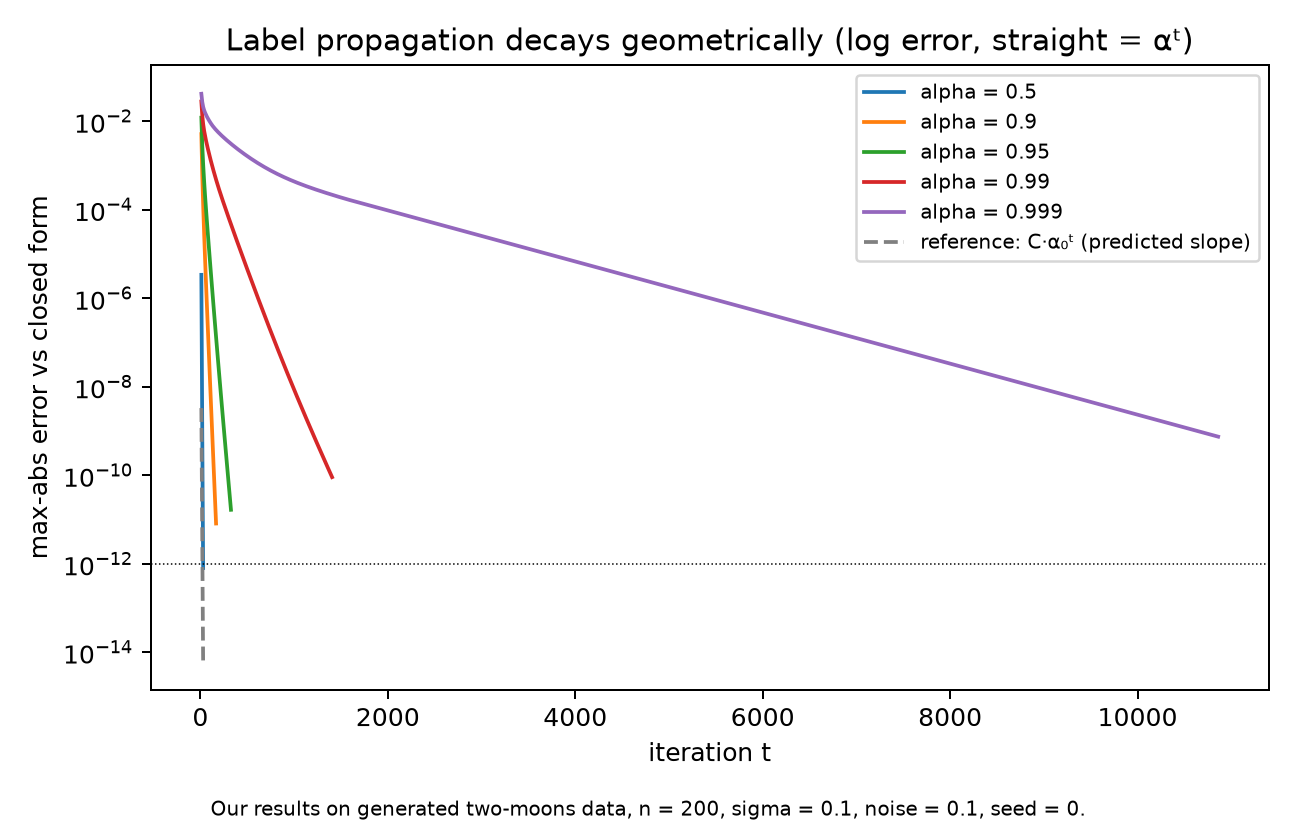
\includegraphics[width=0.72\linewidth]{../results/convergence_rate.png}
  \caption{Log max-abs error of the iteration against the closed form, for four
  values of $\alpha$, on our generated two-moons data. Straight lines confirm the
  geometric decay; the dashed line is the predicted $\alpha_0^{t}$ rate. Our
  result, not the paper's.}
  \label{fig:rate}
\end{figure}

\paragraph{An equation check.}
The last paragraph of Section~2 of the paper claims the transpose variant is
``equivalent'' to $F^{*} = (D - \alpha W)^{-1} D Y$. As written it is not, as
matrices: measured relative gap $0.82$ on our graph. The identity that does hold
(verified to $3\times10^{-15}$) is $(I - \alpha P^{\top})^{-1} Y =
D\,(D - \alpha W)^{-1} Y$ with $P = D^{-1}W$; pre-multiplying by $D$ is a positive
per-row rescaling, so \emph{classifications} agree everywhere and the paper's
word ``equivalent'' is defensible for the argmax rule while the displayed formula
misplaces the $D$ factor. All operator variants ($S$-based, $P$-based,
$P^{\top}$-based, and $(D-\alpha W)^{-1}$ with or without $DY$) differ by at most
$6/200$ predicted points on our toy, a useful robustness observation: the
method's classification is far less sensitive to the normalisation choice than
the raw score matrices are. Full audit in \texttt{results/variants\_audit.csv}.
         % B (written)
% Role C contribution included by main.tex.
% Source: Zhou et al., Sections 4, 4.1--4.3, Figure 5, pp. 324--327.
% Uses bibliography key zhou2003consistency from references.bib.
\subsection{Experimental evidence and its limits}
Zhou et al.~\cite{zhou2003consistency} evaluate their method using a
two-moons illustration, a four-class subset of USPS handwritten digits
(3,874 examples), and four newsgroup topics (3,970 documents represented
by 8,014 features). The real-data comparisons include 1-nearest neighbor,
one-versus-rest RBF SVMs, a harmonic Gaussian field method with class mass
normalization, and two consistency variants. Error is measured on unrevealed
labels, with the digit and text results averaged over 100 trials and at least
one labeled example per class. The consistency methods use $\alpha=0.99$.

Figure~5 of the original paper shows substantially lower digit-recognition
error for the main consistency method than for the supervised baselines.
The text results are more qualified: the harmonic method performs better
at some label budgets. These findings support exploiting unlabeled structure
under the tested conditions, rather than universal superiority over other
semi-supervised methods. The authors' explanation of the harmonic method's
nonmonotonic text results emphasizes the reliability of class-proportion
estimates used in class mass normalization.

A central limitation is model selection. The authors use each algorithm's
respective optimal parameters while acknowledging the difficulty of choosing
parameters with very few labels. The reported comparisons therefore leave
practical label-scarce tuning unresolved. In addition, ensuring label coverage
of every class is a favorable assumption, and the absence of displayed error
bars in Figure~5 limits interpretation of small differences between curves.
These are our assessments of the evidence, not additional experimental findings.

\subsection{Our partial reproduction on two moons}
For each of ten fixed seeds (0--9), we generated 400 two-moons points
with Gaussian coordinate noise of standard deviation 0.08. We revealed one
uniformly sampled label per class and scored predictions on the other 398
points. Euclidean 1-NN and our NumPy LGC implementation used the same
coordinates and revealed labels in each trial.

At our fixed setting of $\sigma=0.15$ and $\alpha=0.99$, mean error across
seeds was $0.45\%$ for LGC (sample SD 0.54 percentage points), compared with
$22.36\%$ for 1-NN (SD 4.22 percentage points). LGC had lower error in every
paired trial. Its per-seed accuracies also matched the independent fixed-point
check described in Section~\ref{sec:theory}.

A descriptive sweep held $\alpha$, data, and revealed labels fixed. LGC mean
error was $0.15\%$, $0.10\%$, $0.45\%$, $14.07\%$, and $32.59\%$ at
$\sigma=0.05, 0.10, 0.15, 0.30,$ and $0.60$, respectively. The results show
that label propagation can exploit the curved structure, and that the
advantage depends on the graph bandwidth. The sweep describes sensitivity
on these trials. Our results concern generated toy data with a label from
each class, so their scope is narrower than the paper's image and text studies.
        % C (written; subsections)
% Section owned by D (Thumula): strengths, limitations, extensions (with C's evidence caveats as input).
\section{Critical discussion}\label{sec:critique}

\emph{[D to write: assumptions of the graph construction, model-selection gap,
sensitivity to $\sigma$, scalability of the dense solve. C's
\texttt{docs/c\_paper\_evidence.md} limitations list is the review-approved raw
material. Target $\approx$0.9 page.] \todo{placeholder}}
       % D
% Shared: 3-4 sentences, agreed by all four at the 28-Nov freeze.
\section{Conclusion}\label{sec:conclusion}

\emph{[To be drafted jointly 25--27 Nov.] \todo{placeholder}}
     % shared, short

\bibliographystyle{plainnat}
\bibliography{references}
% Note: c_references.bib superseded by references.bib (same key zhou2003consistency,
% plus spectral-clustering/harmonic/manifold entries used in the theory section).

\end{document}
